\documentclass{article}
\usepackage[utf8]{inputenc}
\usepackage[right=2cm,left=3cm,top=2cm,headsep=0.5cm,footskip=0.5cm]{geometry}

\title{The Impossible  Early Galaxy Problem}
\author{Santiago Arranz Sanz }
\date{June 2019}

\usepackage{natbib}
\usepackage{graphicx}
\usepackage{latexsym}
\usepackage{eufrak}
\usepackage{dsfont}
\usepackage{hyperref}
\usepackage{enumerate} 
\usepackage{lscape}
\usepackage{titlesec}
\usepackage{fancyhdr}
\usepackage{color}


\newtheorem{teo}{\underline{Teorema}}
\newtheorem{defi}{\underline{Definici\'on}}
\newtheorem{propo}{\underline{Proposici\'on}}
\newtheorem{ejem}{\underline{Ejemplo}}[section]
\newtheorem{prob}{\underline{Problema}}
\newtheorem{lema}{\underline{Lema}}
\newtheorem{obs}{\underline{Observaci\'on}}
\newtheorem{ide}{\underline{Idea}}

\begin{document}

\maketitle

\section*{14/06/2019}

Después de leer varios artículos en los que trata dicho problema y derivados he llegado a la conclusión que el problema base es la discordancia del modelo actual de fusión jerárquica con la falta de observación de galaxias transitorias entre los halos iniciales y las galaxias más masivas en los redshift $z\sim 4-6$. Veamos algunos resumenes de los artículos principales.

\subsection*{The Impossible Early Galaxy Problem}
\citep{steinhardt2016impossibly} Según el paradigma actual de la fusión jerárquica de galaxias en el modelo cosmológico estandar, en torno a los redshift $z\sim 4-6$ ha de existir la transición de las galaxias más masivas desde los halos iniciales que acretan masa a los ultimas fases de evolución bariónica vista en las galaxias con formación estelar y \textit{quasars}. Sin embargo, ninguna evidencia ha sido encontrada en muchos estudios a alto redshift como el CFHTLS, CANDELS y el SPLASH, los primeros estudios para probar la masa alta final en estos redshift. Considerando que el ratio masa halo- masa estelar (SMHMR) estimado a bajo redshift permaneciera constante en $z\sim 6-8$, CANDELS y SPLASH darían mayores ordenes de magnitud de número de halos de masa $M\sim 10^{12-13}M_\odot$ que los que se podrían haber formado a esos redshift, esto se conoce como el problema de la galaxia masiva temprana imposible. En el artículo de \cite{steinhardt2016impossibly} consideran los posibles errores sistemáticos que puedan explicar esta contradicción de teoría y observaciones en los modelos de síntesis estelar usados para estimar los parámetros físicos  y en los escenarios posibles de formación galáctica. Es posible que las incertidumbres desconocidad reduzcan la disparidad entre observaciones y simulaciones de CMD tomando una visión conservadora de las observaciones,aun así existirían tensiones considerables con la teoría.\\


Existe un consenso bastante amplio en la distribución de masa y redshift de los halos producidos en el colapso inicial de las pequeñas fluctuaciones de densidad en el universo temprano y el modelo de fusión jerárquico. Para la cosmología estandar la función de masa es sencilla decalcular. Este consenso se basa en la idea de la rápida evolución en la densidad de halos masivos en $z>4$ que deberían ser observacionalmente evidente en las funciones de masa y luminosidad galácticas. Hasta hace poco el catálogo de galaxias a redshift $z>6$ era limitádo y sesgado a las galaxias más brillantes, galaxas individuales masivas y \textit{quasars}. Sin embargo con los nuevos estudios como el CANDELS o el SPLASH se ha podido probar la función de luminosidad y de masa para galaxias en el rango de $z\sim 4-8$, lo que nos permite calcular la función de masa del halo correspondiente a dicho rango.\\

Trabajos como el de \cite{finkelstein2015increasing} muestra las tensiones ocasionadas en $z>4$ entre la evolución esperada de la función de masa del halo y las funciones de luminosidad y de masa de las galaxias. \\

\subsubsection*{An increasing stellar baryon fraction in bright galaxies at high redshift.}
En el artículo de \cite{finkelstein2015increasing} se centran en el estudio de la función de luminosidad en el UV utilizando observaciones realizadas por el HST con el detector WFC3 y el instrumento IRAC del Spitzer en una muestra de 7500 galaxias con una magnitud alrededor de $M_{UV}^*\simeq -21$ sobre el rango de redshift $z\sim 4-8$, ya que pretenden entender los procesos físicos que regulan la la abundancia de galaxias brillantes en el universo distante. \\

Gracias a los últimos estudios de las pasadas décadas se han facilitado las medidas de la función de luminosidad en el UV, la cual cuantifica las abundacias relativas de galaxias sobre un amplio rango dinámico en luminosidad. Cono la luz UV es un indicador de la actividad de formación estelar, la integral de la función de luminosidad UV es un indicador de la densidad de formación estelar. La función de luminosidad es parametrizada con la función de Schechter de la forma que se ajusta a una ley de potencias en luminosidades bajas y cae exponencialmente en luminosidades altas. Dichos parámetros se corresponden con la luminosidad característica $M_{UV}^*$, la pendiente $\alpha$ y la normalización $\phi^*$. Estudios anteriores vieron que estos parámetros evolucionaban según el redshift, decayendo tanto $M_{UV}^*$ como $\alpha$ según incrementa el redshift. Esta ``evolucion luminosa'' de la función de luminosidad fue ampliamente aceptada como ajuste general de la tendencia observable en la evolución de la densidad de la formación estelar. Sin embargo, trabajos más recientes mostraron que la imagen dibujada era incompleta. Las primeras evidencias vienen de trabajos donde muestran un mayor número de lo esperado de galaxias brillantes sobre redshift $z=7$. \\

Estudios posteriores confirmaron este exceso de galaxias brillantes y concluyeron que no era un efecto atribuible a lentes gravitacionales. Se calculo la función de luminosidad UV y se observo que era contraria a los resultados derivados de conjuntos de datos más pequeños, la luminosidad característica $M_{UV}^*$ era significativamente independiente del redshift entre 4,5,6 y 7. La continuidad del valor de $M_{UV}^*$ se rompe al llegar a $z\sim 8$, donde este cae. Además, mientras que las galaxias en general llegan a ser menos comunes en redshift altos - consistente con la caída en la densidad de la formación estelar- las galaxias brillantes permanecieron relativamente comunes en el universo distante. \textcolor{red}{Esto puede ser posible por un bias observacional, sin embargo no creo que el bias observacional puede explicar que el número de galaxias brillantes permanezca constante, aunque la evolución de la densidad en numero de galaxias en el universo distante no lo ha tratado aún. Si no es un efecto del bias y las galaxias comunes caen en número de densidad mientras que las brillantes se mantienen puede que sea un indicador de que las las galaxias brillantes se formaron primeros y quizás las pequeñas se pudieran formar producto de las interacciónes masivas entre galaxias aunque supongo que es bastante más probable un efecto bias.}\\

En el artículo buscarán los límites de las propiedades físicas en las galaxias brillanes UV distantes e intentarán comprender como ellas mantienen altos niveles de de formación estelar. Los parámetros cosmológicos usados en \cite{finkelstein2015increasing} son los dados por WMAP7, donde $H_0=70.2$ km s$^{-1}$ Mpc $^{-1}$, $\Omega_m=0.275$ y $\Omega_\Lambda=0.725$. De las 7500 galaxias de muestra se centran en 150,75,28,18 y 3 galaxias de $M_{UV}<-21$ en redshift $z=4,5,6,7$ y 8 respectivamente, donde los intervalos de redshift son de un grosor de $\Delta z=0.5$ centrados en los redshift marcados.\textcolor{red}{Dado que los periodos temporales no siguen una relación lineal con el redshift usar un intervalo de redshift constante para todos los casos no debería de ser correcto, ya que un intervalo de $\Delta z=0.5$ en $z=7$ recoge un mayor intervalo temporal que en $z=4$ ¿?}\\

Tras una criba de galaxias tras los ajustes de la distribución espectral de energías (SED) finalmente el estudio se quedan solo con galaxias entre los redshift $z\sim 4-7$. Los parámetros de la mediana del ajuste con un intervalo de confianza de $1\sigma$ no evolucionan significativamente, es decir, podemos hablar en general en redshift $z\sim 4-7$ que las galaxias son moderadamente masivas $\log[M_\star/M_\odot]\sim 9.6-9.9$, algo jóvenes con edades $<100$ Myr, tienen atenuación debida al polvo nada despreciables con $E(B-V)=0.07-0.13$ y alto ratio de formación estelar SFR$\sim 40-60\ M_\odot$ yr$^{-1}$. \textcolor{red}{Lo mas destacable es que no parece haber una relación entre redshift y el valor de estos parámetros, quizás un ligero aumento del SFR, Masa estelar y de la atenuación debida al polvo según decrece el redshift, aunque en muchos casos entran dentro del intervalo de confianza Tabla \ref{tab:finkelstein1}}.\\

\begin{table}[h]
\begin{center}
\begin{tabular}{lccccc}
\hline \hline\\
Redshift & Number & $\log(M_\star/M_\odot)$ & Age & $E(B-V)$ & SFR\\
	&	&	&	(Myr)	&	& $(M_\odot$ yr$^{-1})$\\
\hline\\
z=4 & 94 & 9.86$\pm$0.04 & 44$\pm$2 & 0.13$\pm$0.01 & 56$\pm$4\\
z=5 & 46 & 9.80$\pm$0.06 & 35$\pm$2 & 0.12$\pm$0.02 & 52$\pm$10\\
z=6 & 19 & 9.78$\pm$0.07 & 40$\pm$4 & 0.07$\pm$0.02 & 40$\pm$8\\
z=7 & 14 & 9.64$\pm$0.13 & 29$\pm$8 & 0.09$\pm$0.02 & 41$\pm$9\\
\hline
\end{tabular}
\caption{\label{tab:finkelstein1} Medianas de las propiedades fisicas de galaxias con $M_{UV}<-21$ sacada de \cite{finkelstein2015increasing}}
\end{center}
\end{table}

El paper \cite{finkelstein2015increasing} confirma que las cantidades de polvo observadas en las galaxias masivas/ brillantes en $z=4-7$ son equivalentes. Además, las galaxias menos brillantes y masivas parecen tener menos cantidad de polvo a altos redshift, lo que no es cierto en galaxias brillantes, que confirmó ALMA detectando emisión de polvo en redshift $z\sim 5-7.5$. Si existiera una evolución de la atenuación debida al polvo en las galaxias mas brillantes según evolucione el redshift  podría haber llevado a seleccionar una masa estelar inferior dada una magnitud UV, pero esto no ocurre lo que nos lleva al resultado de que la masa estelar de dichas galaxias brillantes permanecen constante sobre dicho intervalo de redshift. \\

Una pregunta interesante que plantea el artículo de \cite{finkelstein2015increasing} es como las galaxias brillantes en UV en redshift 2-3 están relacionadas con las galaxias brillantes en redshit 6-8. Es decir, desde el punto de vista de la fusión jerárquica, ¿las galaxias brillantes de redshift bajos son descendientes de las galaxias brillantes de redshift altos? ¿Son las galaxias de resdshift altos progenitores de las de redshift bajos? Además, la fusión de galaxias complica la comparación directa basada en el número de densidad de galaxias en cada redshift. Algunos estudios han intentado comparar galaxias en diferentes redshift con el mismo número de denisidad mostrando que tal comparación es adecuada para identificar los descendientes de bajo redshift de poblaciones de altos redshift \textcolor{red}{(Para nuestro caso de galaxias brillantes/masivas)}. Esto es debido a que la mayoría de las galaxias masivas de poblaciones de alto redshift no terminan fusionandose dentro de sistemas más masivos. Sin embargo, el inverso no es cierto. Es decir, el número de desnidad de progenitores en redshift altos de poblaciones de galaxias en bajo redshift son comparablemente mayores a los de estos últimos \textcolor{red}{(Lo que quiere decir es que al contraio que pasa con los descendientes de galaxias masivas, donde el número de densidad se mantiene ya que no ocurren grandes fusiones que aumenten significativamente la masa de estas galaxias masivas a altos redshift, el número de progenitores a alto redshift de galaxias maisvas de bajo redshift es mucho mayor, ya que no solo contribuyen galaxias masivas de alto redshift a la formación de galaxias masivas de bajo redshift, sino la fusiones de galaxias más pequeñas.)}.\\


Las galaxias $M_{UV}<-21$ en $z\sim 2-3$ son los descendientes más plausibles de galaxias de alto redshift más débiles de magnitud, donde concluye el artículo de \cite{finkelstein2015increasing} que comparando galaxias con un brillo similar o galaxias a bajo redsishift con una abundancia similar, las galaxias brillantes UV en $z>6$ son significativamente más jóvenes y menos masivas, pero tienen un SFR similar inferido del brillo simiar en UV y exiben relativamente una evolución escasa de la ateniuación debida al polvo en estos rangos del espectro electromagnético.\\

Con una muestra de galaxias a $z>6$ donde los niveles de SFR y masa estelar se muestran relativamente altos se plantea la posibilidad de que los mecanismos de enfriamiento del gas y su posterior conversión a estrellas difiera de los que ocurren a redshift más bajos. Buscando una respuesta a esta cuestión, se compara la masa estelar $M_\star$ de estos sistemas con la fración de masa bariónica del halo $(\Omega_b/\Omega_m)M_h$ considerando una fración bariónica cósmica $(\Omega_b/\Omega_m)=0.1669$. El agrupamiento de estos sistemas habría proporcionado las restricciones más directas sobre la masa del halo, pero los números y las densidades de la superficie de estas galaxias, en particular a $z> 7$, aún no son suficientes para permitir un análisis de agrupamiento robusto. Por ello, se utuilizó la concordancia de abundancia para estimar las masas de halo para las galaxias brillantes. \\

La concordancia de abundancia supone que la luminosidad de la galaxia o masa estelar sea una función monótona de la masa del halo. Se supone que las galaxias más luminosas viven en los halos más masivos. Este es ciertamente un supuesto plausible entre las galaxias luminosas que se estudian en \cite{finkelstein2015increasing}, pero quizás no lo sea para las galaxias enanas. A partir de las simulaciones de Bolshoi\footnote{Las simulaciones de Bolshoi usa $2048^3$ partículas en un volumen de $250 (Mpc/h)^3$, lo que establece una resolución de $\log(M_h/M_\star)=10$ que es lo suficientemente pequeña para el análisis de las galaxias brillantes/masivas del análisis.} con el modelo $\Lambda$CMD, se selecciona una snapshot cercana al redshift que se pretende estudiar. Una vez identificado los halos virializados se establecen un ranking por masa, para después de ello realizar lo mismo con las galaxias observadas esta vez usando el criterio de luminosidad en vez del de masa y colocar cada galaxia en halo correspondiente a su rango. Este procedimiento es usado para realizar la unión de la estadística de las galaxias con la de los halos.\textcolor{red}{Esta parte no la entiendo muy bien, ¿identifican simplemente las galaxias más luminosas con los halos más masivos? ¿Dos galaxias masivas no pueden pertenecer al mismo halo? Esto daría por defecto un menor ratio de SMHM ya que se impide que las galaxias más masivas estén en halos más masivos.}\\

Por otro lado se usa la parametrización de Shechter vista anteriormente de la fución de luminosidad para establecer la abundancia de galaxias con una magnitud menor a $M_{UV}<-21$ de la muestra analizada. \footnote{Dadas las incertidumbres actuales de la función de masa estelar, trabajar con la función de luminosidad aporta una alternativa mucho más robusta que la masa estelar, aunque en un futuro se debería trabajar con la función de masa estelar ya que ofrece un enlace más directo que la luminosidad en UV.} Comparando dicha función con la función de masa del halo obtenida del promedio en las snapshots seleccionadas en cada rango de redshift obtenemos una función que relaciona la luminosidad de las galaxias con la masa del halo en los que se hospedan, como se ve en la \textbf{Figura \ref{fig:fink1}}. Con este procedimiento se obtiene unas masas de halo de $\log M_h/M_\odot= 11.93, 11.68, 11.57$ y 11.35 en $z=4,5,6,7$ respectivamente, donde los intervalos de confianza los calcularon a traves de 1000 simulaciones MCMC (\textit{Marckov Chain Monte Carlo}) obteniendo margenes de 0.01-0.03 grados de diferencia, lo que son relativamene pequeños dadas las magnitudes consideradas. \textcolor{red}{Aquí vuelve a aparecer la relación galaxias más luminosa halo más masivo dando una relación únivoca entre ambas variables ¿puede que esté aquí el error que desmintiese los resultados contradictorios con la teoría? Debe ser estudiado esta posibilidad.}\\
\begin{figure}[t]
    \centering
    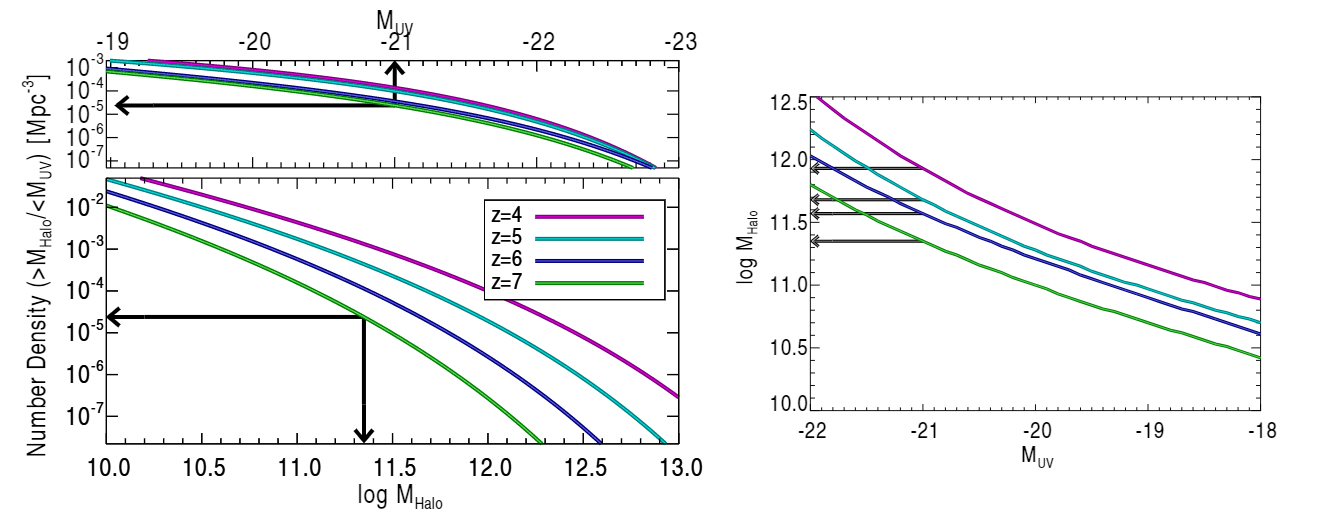
\includegraphics[scale=0.5]{Figuras/fink_1.PNG}
    \caption{Imagen sacada de \cite{finkelstein2015increasing}. Arriba a la izquierda: la función de luminosidad acumulada en z = 4, 5, 6 y 7. Abajo a la izquierda: funciones de masa acumulada del halo en z = 4, 5, 6 y 7, derivadas del promedio de volumen de las funciones de masa de snapshot de Bolshoi en los mismos rangos de redshift como los que definen las muestras de galaxias. Las flechas muestran los resultados de la coincidencia de la abundancia  en z = 7, donde las galaxias con $M_{UV} <-21$, que tienen $n(M_{UV} <-21) = 2.5 \times 10^{-5}Mpc^3$, tienen masas halo de registro $(M_h / M_\odot) = 11.35$. A la derecha: relación entre la magnitud absoluta de UV observada y la masa de halo derivada de la combinación de abundancia en los redshift de interés. Las flechas denotan las masas de halo en la magnitud de interés de $M_{UV} = - 21$.}
    \label{fig:fink1}
\end{figure}

Conociendo los datos de masa estelar de las galaxias con $M_{UV}<-21$ y la masa del halo de las que son huespedes dichas galaxias \cite{finkelstein2015increasing} enfrentan ambos datos en lo que denominan \textit{Stellar Baryon Fraction} (SBF) la cual la defininen como la fración $M_\star/M_h$ de masa estelar del halo versus la masa total (SMHM) en unidades de la fracción demateria bariónica cosmica $(\Omega_b/\Omega_m)=0.1669$. Comparando el SBF con el redsifht se encuentra que existe un aumento a medida que crece el redshift con un valor de $d SBF(z)/dz=0.024\pm 0.007$ como se muestra en la \textbf{Figura \ref{fig:finksbf}}.

\begin{figure}[h]
    \centering
    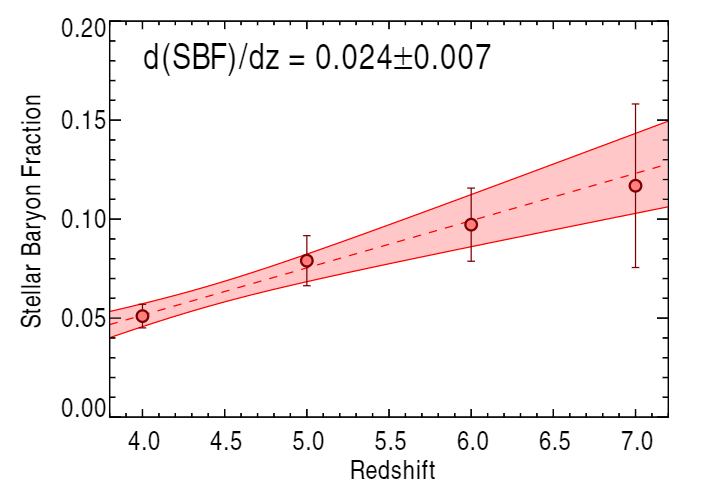
\includegraphics[scale=0.5]{Figuras/sbf.PNG}
    \caption{Imagen sacada de \cite{finkelstein2015increasing}. La (SBF) en galaxias brillantes ($M_{UV} < -21$) de z = 4 a 7. Definimos SBF como la relación de masa estelar a halo en unidades de la fracción de masa de barión cósmica $\Omega_b / \Omega_m$. Encontramos que el SBF aumenta al aumentar el redshift, lo que puede ser responsable de la aparente falta de evolución en la magnitud característica $M^*_{UV}$ observada en este rango de redshift.}
    \label{fig:finksbf}
\end{figure}


\begin{table}[h]
\begin{center}
\begin{tabular}{lcccc}
\hline \hline\\
Redshift & $\log n(M_{UV}<-21)$ & $\log M_h$ & Median & SBF \\
	& (Mpc$^{-3}$)& $(M_\odot)$ &	$M_\star/M_h$	&	\\
\hline\\
z=4 & -3.86 & $11.93_{-0.03}^{+0.03}$ & 0.009$\pm$0.001 & 0.051$\pm$0.006\\
z=5 & -4.01 & $11.68_{-0.03}^{+0.04}$ & 0.013$\pm$0.002 & 0.079$\pm$0.013\\
z=6 & -4.45 & $11.57_{-0.03}^{+0.06}$ & 0.016$\pm$0.003 & 0.097$\pm$0.019\\
z=7 & -4.62 & $11.35_{-0.06}^{+0.09}$ & 0.020$\pm$0.007 & 0.117$\pm$0.043\\
\hline
\end{tabular}
\caption{\label{tab:finkelstein2} Propiedades de los halos de materia oscura de las galaxias estudiadas, sacada de \cite{finkelstein2015increasing}}
\end{center}
\end{table}

Dado que la mediana de las magnitudes de las muestras seleccionadas se encontraban muy cerca del valor $M_{UV}^*=-21$ el estudio decidio volver a calcular la evolución del SBF para magnitudes $M_{UV}=-21\pm 0.25$, de esta manera se obtuvo que la SBF volvía a tener una evolución positiva según crecía el redshift $d SBF(z)/dz=0.0123\pm 0.0041$, una pendiente con un $3\sigma$ de significancia. Con ello concluyeron que el SBF aumentaba con redshift.


\newpage



\bibliographystyle{plainnat}
\bibliography{references}
\end{document}
